\section{Обзор существующих алгоритмов}
\label{sec:Chapter_2} \index{Chapter_2}
\large

\subsection{Модель, основанная на лексико-синтаксических шаблонах}

Данный метод был разработан профессором Марти Херст в 1992 году. Алгоритм является
одним из первых в области автоматического определения отношения обобщения между
словами. Считается, что пара слов в предложении связана отношением гипоним-
гипероним, если она удовлетворяет одному из шаблонов, например, таких как:

\begin{itemize}
\item $[A]$ for example $[B]$ - например
\item $[A]$ such as $[B]$ - такие как
\item $[A]$ include $[B]$ - включая
\item $[A]$ especially $[B]$ - особенно
\end{itemize}

Здесь $[B]$ обозначает \textit{гипероним}, а $[B]$ - список \textit{гипонимов}. Например, <<I like flowers, such as
roses or peonies>> - <<мне нравятся цветы, такие как розы или пионы>>. В данном случае в
качестве гиперонима выступает слово <<цветы>>, а гипонимы - розы и пионы.

Список таких словосочетаний не имеет фиксированного размера. Можно добавлять свои
примеры, подходящие конкретной области или исключать неподходящие.\\

\textbf{ПРЕИМУЩЕСТВА}

\begin{itemize}
\item Высокая точность
\end{itemize}

\textbf{НЕДОСТАТКИ}

\begin{itemize}
\item Главный недостаток такого подхода - низкая полнота определения связей. Необходим
очень большой текстовый корпус, чтобы выделить хотя бы базовые пары отношений.

\item Не каждый пример связи можно описать шаблоном.

\item Не улавливаются цепочки связей. То есть, если определены пары <<ласточка - птица>> и
<<птица - животное>>, то может не быть пары <<ласточка - животное>>.
\item Несмотря на высокую точность, встречаются случаи, когда пара слов неверно отмечена,
как имеющая связь is-a. Один из таких примеров пара предложений:

<<...\textbf{сities} in Asian countries such as \textbf{Tokyo} ...>> - <<... города в странах Азии, такие как Токио
...>>

<<...сities in Asian \textbf{countries} such as \textbf{Japan} ...>> - <<... города в странах Азии, таких как
Япония ...>>

В первом случае пара <<countries - Tokyo>> была бы отмечена неправильно

\item Для ранжирования гиперонимов не достаточно иметь только число, означающее сколько
раз встретилась конкретная пара, так как это зависит от конкретного текстового
корпуса.
\end{itemize}

\subsection{Векторное представление слов}

\subsubsection{Представление слов векторами, полученными при SVM разложении матрицы PPMI}

Данный подход основывается на предположении, которое носит название
<<дистрибутивная гипотеза>>: лингвистические единицы, встречающиеся в схожих
контекстах, имеют близкие значения. Для такого подхода необходимо иметь достаточно
большой текстовый корпус.

Существует несколько способов получение контекстов для слова. Наиболее популярный
называется <<window-based>> метод. Задается величина ширины окна $k$. Далее
просматриваются все предложения, содержащие конкретное слово. К примеру,
интересующее нас слово $W_i$ находится в позиции $i$ в рассматриваемом предложении.
Контекстом данного предложения к $W_i$ будет набор слов ($W_{i-k}, \ldots W_{i-1}, W_{i+1}, \ldots W_{i+k}$) т.е $k$
слов, стоящих до $W_i$ и $k$ слов после. Величина окна произвольная, но чаще всего
выбирается от $2$ до $5$. Таким образом, для каждого слова строится набор его контекстов.

Исследовав схожесть наборов контекстов двух разных слов, можно судить об отношении
этих слов между собой. Например, в случае синонимов, наборы контекстов будут близки.
Задание же функции вычисления схожести является главным параметром таких моделей.

\textit{PPMI} (positive pointwise mutual information) - положительная поточечная взаимная
информация. Функция \textit{PPMI} является одной из оценок схожести двух лингвистических
единиц, например слов, контекстов, абзацев и т.п., на основе заданного текстового
корпуса. Для случая вычисления взаимной информации между словом и контекстом
данная функция задается следующей формулой:

$PPMI (w, c) = max(PMI (w, c), 0)$

$PMI (w, c) = \log \frac{p(w, c)}{p(w) \times p(c)}$, где


\begin{itemize}
\item $w$ - слово из текстового корпуса;

\item $c$ - контекст;

\item $p(w)$ - вероятность встречи слова w в корпусе = частота появления слова в
корпусе деленное на общее число слов

\item $p(c)$ - вероятность встречи данного контекста = частота появления контекста в
корпусе деленное на общее число контекстов

\item $p(w,c)$ - вероятность встречи пары <<слово - контекст>> = частота появления
данной пары в корпусе деленное на общее число пар

\end{itemize}

Таким образом, \textit{PPMI} вычисляется напрямую из текстового корпуса. Если слово и
контекст не связаны между собой, то 

$p(w, c) = p(w) \times p(c)$

и \textit{PPMI} для этой пары будет равно 0. Чем выше данный показатель, тем чаще слово $\mathbf{w}$ появляется в сопровождении
контекста $\mathbf{c}$.

Строится таблица $M$, строки которой соответствуют словам, а столбцы - контекстам.
Таблица заполняется соответствующими значениями \textit{PPMI}. Вектор слова определяется
величинами, расположенными в его строке. Длина вектора - количество найденных в
корпусе контекстов. Таким образом, схожесть наборов контекстов для двух слов
определяется близостью их векторов.

Как можно заметить, величина встречаемости слова намного меньше размера множества
всех контекстов. Значит, матрица $M$ будет иметь большой размер, и при этом она будет
сильно разряженной. Возникает проблема <<проклятия размерности>>. Измерение
расстояния между такими векторами будет неинформативным, т.к согласно Закону
Больших Чисел, сумма $n$ слагаемых стремится к некоторому фиксированному пределу при $n \to \infty$, следовательно, расстояния во всех парах объектов стремятся к одному и тому же значению.

Одним из решений данной проблемы является снижение размерности алгоритмом \textit{SVD}
(Singular Value Decomposition). Данный алгоритм может приблизить матрицу $M$ размера $n \times m$, некоторой другой матрицей $M_k$ с заданным рангом $k$, такой, что её можно разложить в
произведение трех других матриц.

$M \approx M_k = U_k \times \Sigma_k \times V^T_k$,

где $U_k$ и $V_k$ - две унитарные матрицы, состоящие из левых и правых сингулярных
векторов соответственно, а $V^T_k$ - это сопряжённо-транспонированная матрица к $V_k$; $\Sigma_k$ — матрица размера $k \times k$ с неотрицательными элементами, у которой элементы,
лежащие на главной диагонали — это сингулярные числа (а все элементы, не лежащие на
главной диагонали, являются нулевыми)

Полученная матрица $U_k$ будет иметь размерность $n \times k$. Строки такой матрицы будут
соответствовать строкам исходной матрицы $M$, только размерность векторов изменится с
$m$ на $k$. Часть информации потеряется, но существенная её часть остается. Аналогично,
матрица $V^T_k$ несет информацию о столбцах матрицы $M$, только имея при этом меньший
размер.

Применительно к нашей задачи, разложение матрицы \textit{PPMI} приведет к получению
компактного векторного представления слов, сохраняющего информацию о контекстах.

Дальнейшая работа с полученными векторами будет описана в пункте 2.4.


\subsubsection{WORD2VEC}

Еще одним инструментом, реализующим модель векторного представления слов, является
Word2Vec. Этот инструмент был разработан группой исследователей Google в 2013 году,
под руководством Томаша Миколова.

\textit{Word2Vec} реализует две архитектуры - Continuous Bag-of-Words (\textit{CBOW}) и \textit{Skip-gram}. Обе архитектуры построены на нейронных сетях и основаны на дистрибутивной гипотезе.

Принцип работы \textit{CBOW} — предсказывание слова при данном контексте, а \textit{Skip-gram}
наоборот — предсказывает контекст при заданном слове. Независимо от архитектуры,
модель принимает в качестве входных параметров текстовый корпус, и формирует
векторное представление каждого слова, входящего в корпус и имеющего частотность в
заданном диапазоне.

Применяется искусственная нейронная сеть прямого распространения (Feedforward Neural
Network) с функцией активации иерархический софтмакс (Hierarchical Softmax) и/или
негативное сэмплирование (Negative Sampling). Метрика близости векторов – косинусное
расстояние.

Таким образом, данная модель позволяет получить еще одно векторное представление
каждого слова.

\subsubsection{Dynamic distance-margin model}

Две предыдущие модели позволили получить векторные представления слов,
основываясь на наборах их контекстов. При этом каждое слово учитывалось
только один раз, не было различия: слово выступает в качестве гипонима или в
качестве гиперонима.

Отношение is-a не является симметричным. Если пара слов $A-B$ связана
отношением гипоним-гипероним, то пара $B-A$ таким отношением уже не связана.
Более того, чем ближе вектор $A$ к вектору $B$, тем больше вероятность, что слова $А$
и $В$ являются синонимами. Необходимо подбирать границы близости: не слишком
далекие, чтобы слова имели связь друг с другом, и не слишком близкие, чтобы не
получать синонимичные пары. С точки зрения построения моделей, задача поиска
максимума или минимума решается проще и качественнее, чем определение таких
границ. Поэтому возникает предположение о разделение одного вектора слова на
два - вектор гипоним и вектор гипероним.

Вектор слова \textbf{$w$}, используемый, когда данное слово будет выступать в качестве
гипЕронима, обозначим за \textbf{$E(w)$}. Например, слово \textit{птица} в отношении (\textbf{ласточка}, \textbf{птица}). Когда в качестве гипОнима - за \textbf{$O(w)$}. Пример: в паре (\textit{птица}, \textit{животное}).

Предполагается, что построенная новая модель должна удовлетворять следующим
трем правилам:

\begin{enumerate}
\item Если пара слов $u-v$ связана отношением гипоним-гипероним, то вектора $O(u)$ и $E(v)$ находятся близко друг к другу. $O(u) \approx E(v)$.

\item Если пара слов $u-v$ являются ко-гипонимами, т.е. существует слово $w$,
являющееся гиперонимом, как для слова $u$, так и для слова $v$, то должно
выполняться соотношение $O(u) \approx O(v)$.

\item Аналогично, если пара слов является ко-гиперонимами, то должно быть верно: $Е(u) \approx Е(v)$.
\end{enumerate}

Таким образом задача сводится к минимизации расстояний $O(u) \approx E(v)$, $O(u) \approx O(v)$ и $Е(u) \approx Е(v)$.

В качестве обучающего множества берется набор триплетов $(u, v, q)$, где $u$ - гипоним, $v$ - гипероним, а $q$ - сколько раз пара гипоним-гипероним $(u, v)$ встретилась в текстовом корпусе. Такой набор данных может быть собран вручную или,
например, методом шаблонов, описанным в пункте 2.1. Необходимо учитывать, что
для получения хороших результатов, размер текстового корпуса должен быть
очень большим.

Для каждой пары $x = (u, v, q)$ из выбранного набора данных, вычисляется функция
расстояния между векторами $O(u)$ и $E(v)$. В качестве функции расстояния может,
например, выступать 1-норма разности векторов. Так

$f(x) = ||O(u) - E(v)||_1$

Для того, чтобы оценить величину ошибки модели на примере $x$, расстояние между
векторами слов $u$ и $v$ сравнивается с расстоянием от $u$ до произвольного слова $v'$.
Т.е выбирается негативный пример гиперонима для гипонима $u$. По
предположению, построенные вектора $O(u)$ и $E(v)$ должны быть ближе, чем
вектора $O(u)$ и $E(v')$. Насколько ближе они должны быть, определяется величинамиq и $q'$. Величина $q'$ означает, сколько раз пара гипоним-гипероним $(u, v')$
встретилась в текстовом корпусе. Так как слово $v$ выбирается случайным из всего
корпуса, то наиболее вероятно $q$ равняется нулю.

Величины $q$ и $q'$ показывают насколько вероятным может быть существование
отношения is-a между соответствующими им парами слов. Тогда, чем больше
разница этих вероятностей, тем расстояния между величинами $f(x)$ и $f(x')$ должно
быть больше. Учитывая проведенный анализ, вводятся следующие соотношения:

\begin{itemize}
\item $x' =$ \textit{триплет} $(u, v', q')$

\item $f(x) < f(x') - m(q, q')$

\item $m(q, q') = log(q + 1) - log(q' + 1) = log \frac{q + 1}{q' + 1}$
\end{itemize}


В таком случае, ошибку модели на примере $x$ можно вычислить как

$$max(0, f(x) - f(x') + m(q, q') )$$

И тогда модель будет обучаться уже на парах $(x, x')$.
Аналогично, в качестве негативного примера $x'$ может выступать не только триплет
$(u, v', q')$, но и $(u', v, q')$.

Для того, чтобы обучать модель чаще на парах, которые с большей вероятностью
имеют отношение is-a, используется искусственное увеличение обучающего
множества пар $(x, x')$ с учетом этой вероятности. Для каждого триплета $x$
подбирается столько негативных примеров $x'$, сколько раз $(u, v)$ встретилась в
текстовом корпусе, т.е создается $q$ различных пар $(x, x')$.
Итоговая функция потерь построенной модели вычисляется как:

$$\sum_{x = (u, v, q)} \sum_{j = 1}^{q} max(0, f(x) - f(x'_j) + m(x, x'_j))$$

При успешном обучении данной модели, она будет удовлетворять всем трем
условиям, описанным выше:

\begin{enumerate}
\item $O(u) \approx E(v)$ достигается за счет непосредственной минимизации расстояния $f(x)$
\item Если для пары $(u, v)$ существует слово $w$, являющееся гиперонимом, как для
слова $u$, так и для слова $v$, то из первого пункта следует: $O(u) \approx E(w)$ и $O(v) \approx E(w)$, а значит, и $O(u) \approx O(v)$. Другими словами, оба слова $u$ и $v$ подтягиваются к
слову $w$, тем самым становясь ближе друг к другу.
\item Аналогично достижима цель $Е(u) \approx Е(v)$
\end{enumerate}

Выполняя все эти 3 условия, становится возможным определение пары (ласточка,
животное) имея в изначальном наборе данных только пары (ласточка, птица) и
(птица, животное). Устранился один из важных недостатков чисто шаблонных
моделей.

Обучение такой модели сводится к обучению нейронной сети, имеющей
следующую архитектуру:

\begin{figure}[H]
\centering 
    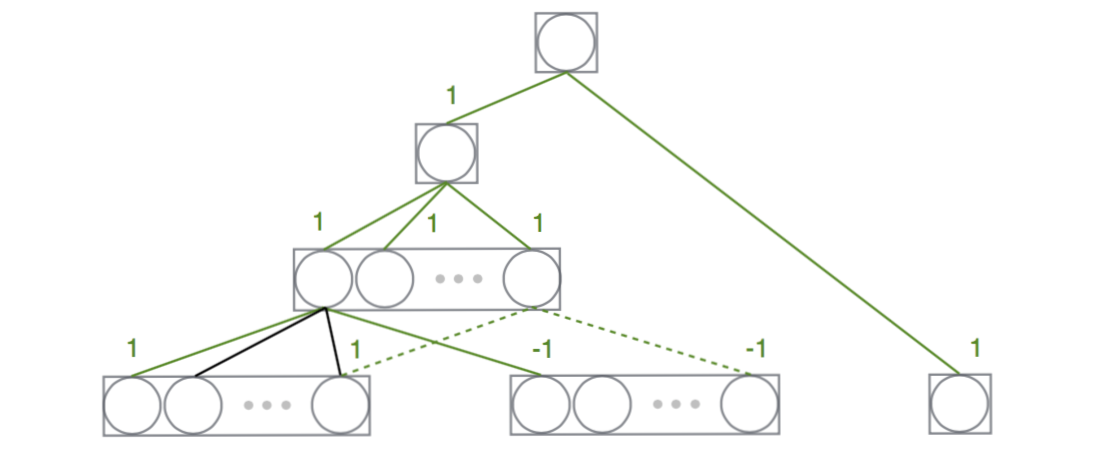
\includegraphics[scale=0.6]{image/NN_part1_new.png}
    \caption{$p(x)$ - вычисление расстояния между векторами $O(u)$ и $E(v)$ для $x = (u, v, q)$.}
    \label{srg}
\end{figure}

\begin{figure}[H]
\centering 
    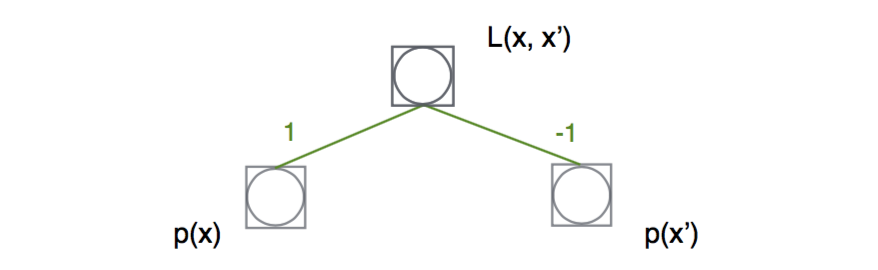
\includegraphics[scale=0.6]{image/NN_part2_new.png}
    \caption{$L(x, x’)$ - вычисление ошибки для триплета x и его негативного примера $x’$.}
    \label{srg}
\end{figure}

\begin{figure}[H]
\centering 
    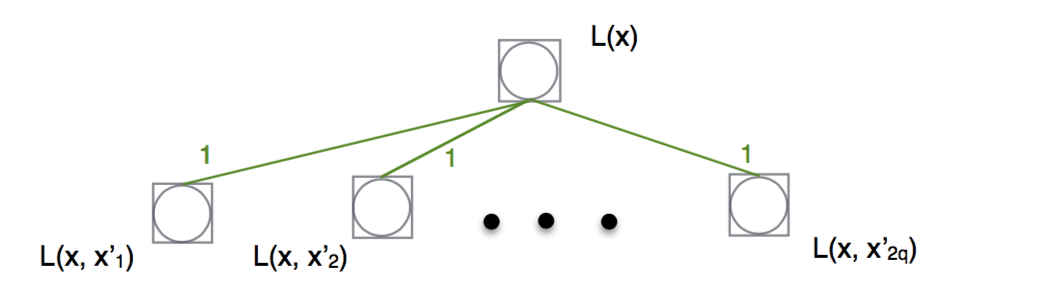
\includegraphics[scale=0.6]{image/NN_part3_new.png}
    \caption{$L(x)$ - вычисление суммарной ошибки для триплета $x$.}
    \label{srg}
\end{figure}

\begin{figure}[H]
\centering 
    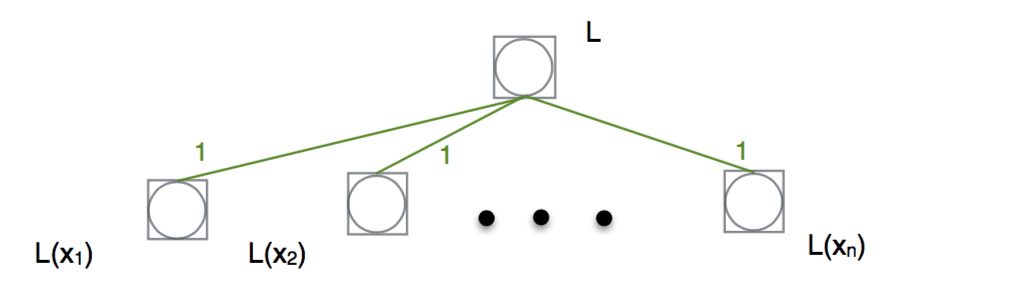
\includegraphics[scale=0.6]{image/NN_part4_new.png}
    \caption{$L$ - вычисление функции потерь модели.}
    \label{srg}
\end{figure}

Модель оптимизируется алгоритмом $SGD$.

Таким образом, разобраны три различные модели получений векторов слов.
Осталось рассмотреть способы вычисления итоговых предсказаний существования
отношений \textit{is}-a между словами, используя их векторное представление.



\subsubsection{Обучение модели, предсказывающей существование связи IS-A, на основе векторов слов.}

Как было сказано, большинство задач, связанных с темой определения
существования связи \textit{is}-a, были сведены к выставлению каждой паре слов либо 0
(связи нет), либо 1 (при её наличии). Поэтому чаще всего для последующего
обучения векторов был выбран алгоритм $SVM$.

Для обучения брался готовый размеченный корпус пар слов, имеющих между
собой отношение гипоним-гипероним, и подмешивался к нему набор пар, не
имеющих такой связи. Все, что оставалось, это скомбинировать вектора слов из
пары, в качестве входного вектора для обучения.

Существует множество различных комбинаций. Наиболее используемые из них
следующие:

\begin{itemize}
\item Разность векторов $<u - v>$
\item Соединение векторов (конкатинация) $<u, v>$
\item Вычисление косинусного расстояния $cos(u, v)$
\item Евклидово расстояние $|| u - v ||_2$
\item И их комбинации, например:
\begin{itemize}
\item конкатенация с добавлением евклидового расстояния

$<u, v, || u - v ||_2>$
\item разность векторов с добавлением косинусного расстояния

$<u - v, cos(u, v)>$
\end{itemize}
\end{itemize}

Таким образом для каждой из трех моделей получения векторного представления
слов, выбирался какой-то из способов комбинирования векторов и происходило
обучение на таких входных данных алгоритма $SVM$.

Как показали эксперименты, такие виды моделей давали показатели метрик
классификации лучше, по сравнению с чисто шаблонными методами.